\chapter{Probabilistic Model of Linear Regression}
\section{Introduction}

The probabilistic model of linear regression provides a way to understand and interpret linear regression models from a probabilistic view. \\

Consider training data $\D$ :
$$
  \D = \{(\x_i,y_i)\}_{i=1}^n
$$

\tc{Assumption}: The relation between the input features $\x$ and the target $y$ can be represented by a linear equation with some added noise $\epsilon$:
$$
  y_i = \w^T\x_i + \epsilon_i
$$

\tc{Noise}: The noise component $\epsilon$ signifies the fluctuation within the data that contributes towards uncertainty in the target values and cannot be explained by the linear relationship. Assume that it follows a Gaussian distribution with mean 0 and variance $\sigma^2$
$$
  \epsilon_i \sim \mathcal{N}(0, \sigma^2)
$$

In other words, $\epsilon_i$'s are independent and identically distributed (i.i.d.) Gaussian random variables with zero-mean and the same variance $\sigma^2$. Now, we can represent target $y_i$ as a Gaussian distribution with mean $\w^T\x_i$ and variance $\sigma^2$
$$
  y_i \sim \mathcal{N}(\w^T\x_i, \sigma^2)
$$

Given training data $\D = \{(\x_i, y_i)\}_{i=1}^{n}$ where feature vector $\x_i \in \mathbb{R}^{d}$, target $y_i \in \mathbb{R}$,
$$
  P(y_i \mid \x_i, \w)=\frac{1}{\sqrt{2\pi}\sigma} e^{-\frac{(y_i - \w^T\x_i)^2}{2\sigma^2}}
$$
$$
  \text{Likelihood : } \quad P(y_1, y_2, \ldots, y_n \mid \x_1, \x_2, \ldots, \x_n) = \pi_i P(y_i \mid \x_i, \w)
$$
$$
  \text{Log Likelihood : } \quad \log P(y_1, y_2, \ldots, y_n \mid \x_1, \x_2, \ldots, \x_n) = \underset{i}{\sum} \log P(y_i \mid \x_i, \w)
$$

The likelihood function models how well the observed data fits the assumed model. In case of linear regression, it measures the probability of observing the actual target values given the parameter vector w and feature vectors.

\section{Maximum Likelihood Estimation}

The process of finding the best-fitting model often involves estimating the model's parameters in a way that maximizes the likelihood of observing the actual data. This estimation process is known as Maximum Likelihood Estimation (MLE). It is a \textit{Frequentist} view in machine learning. \\

For the model, $y_i$(target value) represented as a Gaussian distribution $\mathcal{N}(\w^T\x_i, \sigma^2)$, the parameter of interest is the weight vector $\w$. We need to find $\w$ that maximizes the likelihood function. Maximizing likelihood function is equivalent to maximizing log likelihood function. (The $\log$ function is strictly increasing, and thus maximizing the log likelihood gives the same solution as maximizing the likelihood function.)
$$
  \w_{\text{MLE}} = \argmax_{\w} \underset{i}\sum \log P(y_i \mid \x_i, \w)
$$

\subsection{Motivating Example}
You want to estimate the probability of a biased coin landing on heads. The probability that the outcome is head for a coin toss is $\theta$.  Let us say your data contains $N$ coin tosses with $N_H$ heads and $N_T$ tails. What is the maximum likelihood estimate of $\theta$ ?\\

Likelihood function: probability of data, given parameter $\theta$
\begin{align*}
  P(D\mid\theta)               & = \theta^N_H(1-\theta)^N_T                                              \\
  \implies \theta_{\text{MLE}} & = \argmax_{\theta} \log P(\D \pipe \theta)                              \\
                               & = \argmax_{\theta} \log \left( \theta^{N_H} (1-\theta)^{N_T} \right)    \\
                               & = \argmax_{\theta} \left( N_H \log \theta + N_T \log (1-\theta) \right)
\end{align*}

To find $\theta_{\text{MLE}}$, we need to find the derivative of $N_H \log \theta + N_T \log (1-\theta)$ w.r.t. $\theta$, set to zero and solve for $\theta$:
\begin{align*}
  \frac{N_H}{\theta_{\text{MLE}}} & - \frac{N_T}{1-\theta_{\text{MLE}}} = 0 \\
  \implies \theta_{\text{MLE}}    & =\frac{N_H}{N_H+N_T}=\frac{N_H}{N}
\end{align*}

\subsection{Question}
Say you have a coin with P $\in$ \{0.4,0.6\} \\
Data: 3 coin tosses; 2 heads, 1 tail \\
What is MLE of P ? \\

\tc{Solution}:
\begin{align*}
  P(D\mid\theta)_{\theta = 0.4} & = (0.4)^2 (0.6)                 \\
  P(D\mid\theta)_{\theta = 0.6} & = (0.6)^2 (0.4)                 \\
  P(D\mid\theta)_{\theta = 0.6} & > P(D\mid\theta)_{\theta = 0.4} \\
  \tc{Answer}                   & = 0.6
\end{align*}

\subsection{MLE for linear regression}
\begin{align*}
  w_{\text{MLE}} & = \argmax \sum_i \log P(y_i \mid \x_i, \w)                                                  \\
                 & = \argmax \sum_i \log ( \mathcal{N}(\w^T\x_i, \sigma^2))                                    \\
                 & = \argmax \sum_i \log \frac{1}{\sqrt{2\pi}\sigma} e^{-\frac{(y_i - \w^T\x_i)^2}{2\sigma^2}} \\
                 & = \argmax C - \sum_i {\frac{(y_i - \w^T\x_i)^2}{2\sigma^2}}                                 \\
  w_{\text{MLE}} & = \argmin \sum_i {(y_i - \w^T\x_i)^2}
\end{align*}

\begin{itemize}
  \item MLE under Gaussian noise distribution is equivalent to the least squares solution.
  \item MLE under Laplacian noise distribution is equivalent to Least Absolute Deviation solution.
  \item A significant drawback of Maximum Likelihood Estimation (MLE) arises when working with limited data, as it can lead to overfitting due to its heavy reliance on the available dataset.
\end{itemize}

\section{Bayesian Parameter Estimation}
In MLE, observations are random variables while parameters are not. On the contrary, in the Bayesian framework, parameters are also treated as random variables alongside observations. Parameters have an underlying \tc{prior distribution} which encode beliefs prior to observing the data. As MLE has a high tendency to overfit, we switch to a different estimation, namely the \tc{Maximum Aposteriori Estimation} with the hope of alleviating overfitting using prior information.

\section{Maximum Aposteriori Estimate ( MAP )}

Maximum A Posteriori (MAP) estimation focuses on incorporation of prior knowledge into estimating the underlying model parameters which are denoted by $\Theta$. We assume a prior distribution $\Pb(\Theta)$ for parameters $\Theta$ (before observing the data $\D$). \\

By Bayes' theorem, we have :
$$
  \Pb(\Theta \pipe \D) = \frac{\Pb(\D \pipe \Theta)\Pb(\Theta)}{\Pb(\D)}
$$

$\bm{\Pb(\Theta \pipe \D)}$ is the \tc{posterior} probability for the model parameters $\Theta$ given data $\D$. \\
$\bm{\Pb(\D \pipe \Theta)}$ is the \tc{likelihood} of observing the data given model parameters \& $\bm{\Pb(\Theta)}$ is the \tc{prior}.
\begin{align*}
  \Theta_{\text{MAP}} & = \arg \max\limits_{\Theta} \Pb(\Theta \pipe \D)                             \\
                      & = \arg \max\limits_{\Theta} ( \log \Pb(\D \pipe \Theta) + \log \Pb(\Theta) )
\end{align*}

\tc{Note:} The posterior is directly proportional to the product of likelihood and the prior functions as shown by the following equation,
\begin{align*}
  \Pb(\Theta \pipe \D) & \propto  \Pb(\D \pipe \Theta)  \Pb(\Theta)           \\
                       & \propto \log \Pb(\D \pipe \Theta) + \log \Pb(\Theta)
\end{align*}

\subsection{Coin example (MAP estimate)}

Suppose, we have a biased coin and N\textsubscript{H} and N\textsubscript{T} are the number of heads and tails obtained.\\ Likelihood ($\Pb\D \pipe \Theta$) , i.e, the probability of data given the parameter $\Theta$ is given by the following equation,
$$
  \Pb(\D \pipe \Theta)=\Theta^{N_H}(1-\Theta)^{N_T}
$$

What is a good prior on $\Theta$ ? \\
\tc{Beta distribution} is a good candidate for prior because the functional form of prior matches with that of the likelihood.
\begin{align*}
  \Beta(\Theta,\alpha,\beta) = c\,\Theta^{\alpha-1}(1-\Theta)^{\beta-1} &  & [c= \frac{\Gamma(\alpha + \beta)}{\Gamma(\alpha)\Gamma(\beta)},\; \Gamma(.) \text{ is the gamma function} ]
\end{align*}

Hence, the posterior will be
\begin{align*}
  \Pb(\Theta,\D) & \propto \Pb(\D \pipe \Theta) \Pb(\Theta)                 \\
                 & \propto c\,\Theta^{N_H+\alpha-1}(1-\Theta)^{N_T+\beta-1} \\
                 & \propto \Beta(\Theta,N_H+\alpha,N_T+\beta)
\end{align*}

\section{Conjugate Priors}
For a likelihood P($\D \pipe \Theta$) coming from a family of distributions $d_{1}$, a prior (from a family $d_{2}$) is said to be a conjugate prior if the posterior distribution also comes from the family $d_{2}$. ($d_{2}$ could also be from the same family as $d_{1}$).

\subsection{Coin example}
Continuing with the coin example mentioned above, the probability of getting N\textsubscript{H} heads and N\textsubscript{T} tails upon tossing a biased coin with the probability of getting head as $\Theta$ (Bernoulli distribution), is given by,
$$
  \Beta(N\textsubscript{H}, N\textsubscript{T}, \Theta) = \Theta^{N\textsubscript{H}}(1-\Theta)^{N\textsubscript{T}}
$$

Also, the PDF for beta distributions is given as,
$$
  \Beta(\Theta, \alpha, \beta) = c.\Theta^{\alpha - 1}(1-\Theta)^{\beta - 1}
$$

The posterior is proportional to the product of likelihood and prior and putting their values we have,
\begin{align*}
  P(\Theta \pipe \D) & \propto  P(\D \pipe \Theta)  P(\Theta)                                                      \\
                     & \propto \Theta^{N\textsubscript{H} + \alpha - 1}(1-\Theta)^{N\textsubscript{T} + \beta - 1} \\
                     & \propto \Beta(\Theta, N\textsubscript{H} + \alpha, N\textsubscript{T} + \beta)
\end{align*}

Hence,
$$
  \Theta_{MAP} = \argmax ((N_H+\alpha-1)\log(\Theta) + (N_T+\beta-1)\log(1-\Theta))
$$

On maximizing it, we get
\begin{align*}
  \frac{N_H+\alpha-1}{\Theta} & - \frac{N_T+\beta-1}{1-\Theta} = 0            \\
  \implies \Theta_{MAP}       & = \frac{N_H+\alpha-1}{N_H+N_T+\alpha+\beta-2}
\end{align*}

Compared to the MLE estimate $\Theta_{\text{MLE}} = \frac{N_H}{N}$, MAP estimate has extra counts denoted by $\alpha$ and $\beta$. \\

We can see that as $N \to \infty \Theta_{\text{MAP}}$ converges to $\Theta_{MLE}$. This represents the fact that prior beliefs become less representative over more data. This is encapsulated in the \href{https://en.wikipedia.org/wiki/Bernstein\%E2\%80\%93von\_Mises\_theorem}{Bernstein - von Mises Theorem}. Further, we also see that in essence, the prior data is enforcing a belief of a ``pre-existing" $\alpha - 1$ heads out of $\alpha + \beta - 2$ tosses. For this reason, these numbers can also be thought of as pseudo coin counts. \\

\tc{Additional Note}: There are a large number of exponential families that serve as conjugate priors for different distributions due to their exponential mathematical form.
\begin{enumerate}
  \item Beta distribution serves as conjugate prior for Bernoulli \& Binomial likelihoods.
  \item Normal distribution is a conjugate prior for itself, i.e. a Gaussian distribution is a conjugate prior for other Gaussian likelihoods, however, inverse gamma distribution also is a conjugate prior for Gaussian likelihood.
  \item Dirichlet prior is used as conjugate for Multinomial distributions.
\end{enumerate}

\subsection{Linear Regression MAP Estimate}

Given the probabilistic setup of Linear Regression, we try to estimate the weights $\w$.

Let's consider zero mean Gaussian Prior on the weights $\w$ with covariance matrix as scaled identity matrix, i.e.
\begin{align*}
  \mathcal{P}\left(\w\right) & = \mathcal{N}\left(0,\frac{\mathbf{I}}{\lambda}\right)                                                                                    \\
                             & = \frac{1}{(2\pi)^{d/2}\sqrt{\det(\mathbf{I}/\lambda)}} \exp{\left(-\frac{1}{2}\w^T\left(\frac{\mathbf{I}}{\lambda}\right)^{-1}\w\right)} \\
                             & = \left(\frac{\lambda}{2\pi}\right)^{d/2} \exp{\left(-\frac{\lambda}{2}\w^T\w\right)}                                                     \\
                             & = \left(\frac{\lambda}{2\pi}\right)^{d/2} \exp{\left(-\frac{\lambda}{2}\norm{\w}_2^2\right)}
\end{align*}

Now, if we try to find the MAP estimate for $\w$,
\begin{align*}
  \w_{\text{MAP}} & = \underset{\w}{\arg\max}
  \bigl(\mathcal{P}\left( \D \, | \, \w\right) \, \mathcal{P}\left(\w\right)\bigr) \\
                  & =\underset{\w}{\arg\max}
  \Bigl(\log\bigl(\mathcal{P}\left( \D \, | \, \w\right)\bigr) + \log\bigl(\mathcal{P}\left(\w\right)\bigr)\Bigr)
\end{align*}

Using the MLE equation to rewrite the log-likelihood term and plugging in the prior term gives us,
\begin{align*}
  \w_{\text{MAP}} & = \underset{\w}{\arg\max}
  \left(\frac{-1}{2\sigma^2} \sum_{i=1}^n \left(y_i - \w^T\x_i\right)^2 + \frac{d}{2}\log\left(\frac{\lambda}{2\pi}\right) - \frac{\lambda}{2}\norm{\w}_2^2\right) \\
                  & = \underset{\w}{\arg\min}
  \left(\frac{1}{2\sigma^2} \sum_{i=1}^n \left(y_i - \w^T\x_i\right)^2 + \frac{\lambda}{2}\norm{\w}_2^2\right)
\end{align*}

Recall that this is same as the $L_2$-regularised linear regression (or Ridge Regression).\\

\tc{NOTE}: By changing the prior, we can get various types of regularisations. For example, using a Laplace Prior will give \(L_1\) Regularisation (or Lasso Regression)

\section{Bias and Variance of Estimates}
Natural question that arises after creating different types of Linear Regression models is that "How do we evaluate whether the predictor is good or not?". \\

One of the metric that we use to generate the model is Training Loss, but this does not tell whether the model will be able to generalize or not. Hence, to define whether a model is good or not, we look at the Test Loss. \\

So, we try to decompose the Expected Test Loss and it turns out that it has 3 components
\begin{enumerate}
  \itemsep-0.3em
  \item Variance
  \item Bias
  \item Noise (or Irrecoverable error/ Unavoidable error)
\end{enumerate}

Out of these, Variance and Bias are inherent to the model and Noise is inherent to the data (due to inaccuracies in measurements).

\subsection{Bias}

Let us assume that we are sampling data from a true distribution
$$
  y = f(\x) + \epsilon
$$

where $\epsilon$ is a zero mean Gaussian Noise with standard deviation $\sigma$. Let $h_{\w}(.)$ be the predictor for a given data $\D$. Then the bias of the given model for a particular $\x$ can be defined as follows
$$
  \text{Bias} = \mathbb{E}\left[h_\w(\x)\right] - f(\x)
$$

Note that the expectation is over various choice of training data set $\D$ which will give rise to various $h_\w(.)$. Also, $\x$ is fixed value and the expectation does not depend on it.
To explain the meaning of bias, let us sample multiple different data sets from the given true distribution and find the predictor function for each of them. Then the bias represents how close the average of these predictor functions is to the true distribution.

\begin{figure}[H]
  \centerline{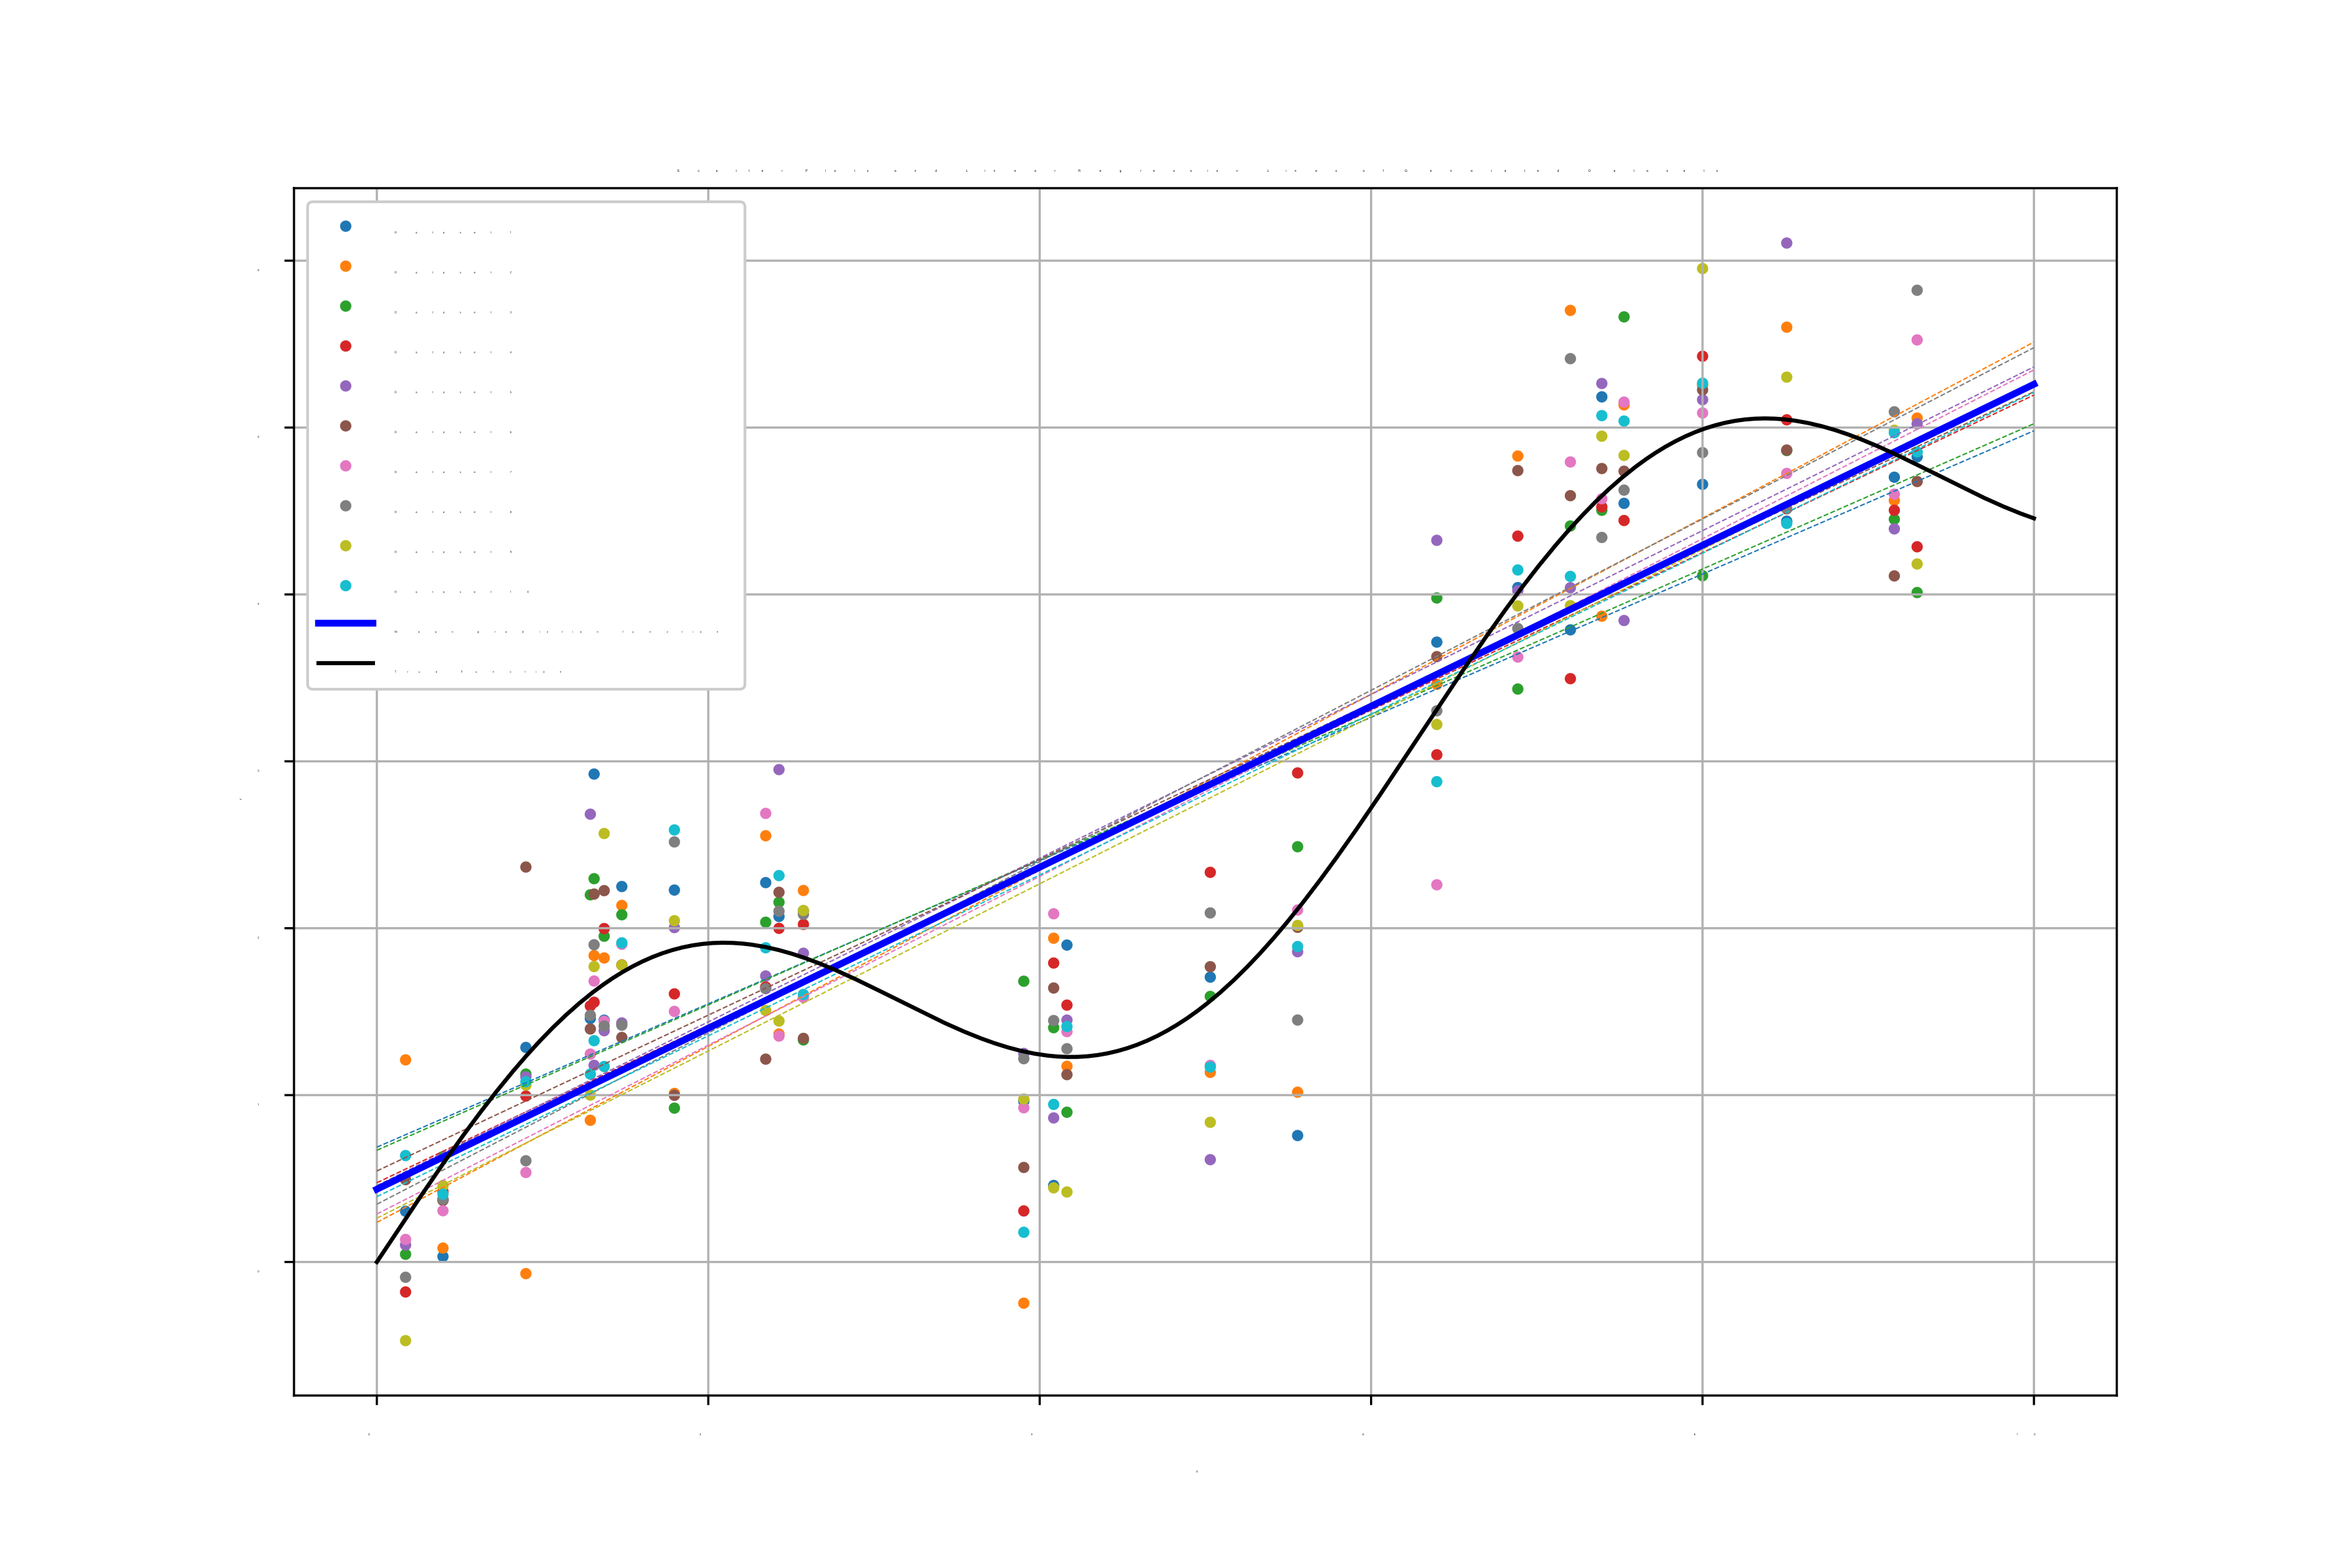
\includegraphics[width = 0.7\textwidth]{images/13.png}}
  \caption{Showing various regression arising from various data-sets and the mean of them}
  \label{fig}
\end{figure}

\subsection{Variance}

Considering the same setup as before, the variance of the given model for a particular \(\x\) can be defined as follows
\begin{equation}
  \text{Variance} = \mathbb{E}\left[\bigl(h_\w(\x)-\mathbb{E}\left[h_\w(\x)\right]\bigr)^2\right]
\end{equation}
Note that the expectation is over various choices of training data set \( \D\) which will give rise to various \(h_\w(.)\). Intuitively, variance of given model is basically the variance of different predictor functions that we get by varying the data set \( \D\). Qualitatively, it measures the spread of predictor functions in figure \ref{fig}.

\subsection{Noise}

Noise is the unavoidable error in the data caused by the errors in measurement. The expression for this error is as follows
\begin{equation}
  \text{Noise} = \mathbb{E}\left[\bigl(y-f(\x)\bigr)^2\right]
\end{equation}
Note that this expectation is over the random noise (i.e. $\epsilon$ in this case) and not dependent on the data set. This reduces to
\begin{align*}
  \text{Noise} & = \mathbb{E}\left[(\epsilon)^2\right] \\
               & = \text{Var}(\epsilon)                \\
               & = \sigma^2
\end{align*}

\subsection{Analysing Unregularized Linear Regression}

Let us assume that we have the same model as before, i.e.
$$
  y = f(\x) + \epsilon \;\;\text{and}\;\; \epsilon \sim \mathcal{N}(0,\sigma^2)
$$

As mentioned before, we are trying to find the expected test error. Let us denote the test data point as $(\widetilde{\x},\widetilde{y})$ i.e. $\widetilde{y} = f(\widetilde{\x}) + \widetilde{\epsilon}$. Then we have to find
$$
  E_{\text{test error}} = \mathbb{E}_{\widetilde{\epsilon},\D}\left[\bigl(\widetilde{y} -h_\w\left(\widetilde{\x}\right)\bigr)^2\right]
$$

\tc{NOTE}: Here, we are assuming that $\xt$ is a constant while taking the expectation, i.e. LHS should ideally be parameterized as $E_\text{test error}(\xt)$. This would also mean that $\yt$ (which is a random variable) is only dependent on $\widetilde{\epsilon}$.
\begin{align*}
  E_{\text{test error}} & = \mathbb{E}\left[\bigl(\widetilde{y} -h\left(\widetilde{\x}\right)\bigr)^2\right]                                                                \\
                        & = \expe{\yt^2} + \expe{\hxt^2} - 2 \, \expe{\yt} \, \expe{\hxt}                                                                                   \\
                        & = \expe{\bigl(\yt - \expe{\yt}\bigr)^2} + \expe{\yt}^2 + \expe{\bigl(\hxt - \expe{\hxt}\bigr)^2} + \expe{\hxt}^2 - 2 \, \expe{\yt} \, \expe{\hxt} \\
                        & = \expe{\bigl(\yt - f(\xt)\bigr)^2} + \expe{\bigl(\hxt - \expe{\hxt}\bigr)^2} + \expe{\hxt}^2  + \expe{\yt}^2 - 2 \, \expe{\yt} \, \expe{\hxt}    \\
                        & = \expe{\bigl(\yt - f(\xt)\bigr)^2} + \expe{\bigl(\hxt - \expe{\hxt}\bigr)^2} + \Bigl(\expe{\hxt}  - \expe{\yt}\Bigr)^2                           \\
                        & = \expe{\bigl(\yt - f(\xt)\bigr)^2} + \expe{\bigl(\hxt - \expe{\hxt}\bigr)^2} + \Bigl(\expe{\hxt}  - f(\xt)\Bigr)^2                               \\
                        & = \text{Noise} + \text{Variance} + \text{Bias}^2
\end{align*}

\begin{mdframed}
  \tc{Explanations of steps}:
  \begin{itemize}
    \item The predicted value $h(\xt)$ depends only on the data set and hence it is independent of the actual value $\yt$ (which is only dependent on $\widetilde{\epsilon}$)
    \item Using the definition of variance we can get $\expe{Y^2} = \expe{\bigl(Y-\expe{Y}\bigr)^2} + \expe{Y}^2$
    \item Also, note that $\expe{\yt} = \expe{f(\xt)+\widetilde{\epsilon}} = \expe{f(\xt)}+\expe{\widetilde{\epsilon}} = f(\xt)$ as the noise is zero mean and $\xt$ is a constant (as mentioned before)
  \end{itemize}
\end{mdframed}

\pagebreak
\subsection{Variance-Bias Trade-Off}

Let us look at the use of the above-mentioned formula. \\

Consider the following case where we have used a very high complexity model for linear regression.

\begin{figure}[H]
  \centering
  \begin{subfigure}{.4\textwidth}
    \centering
    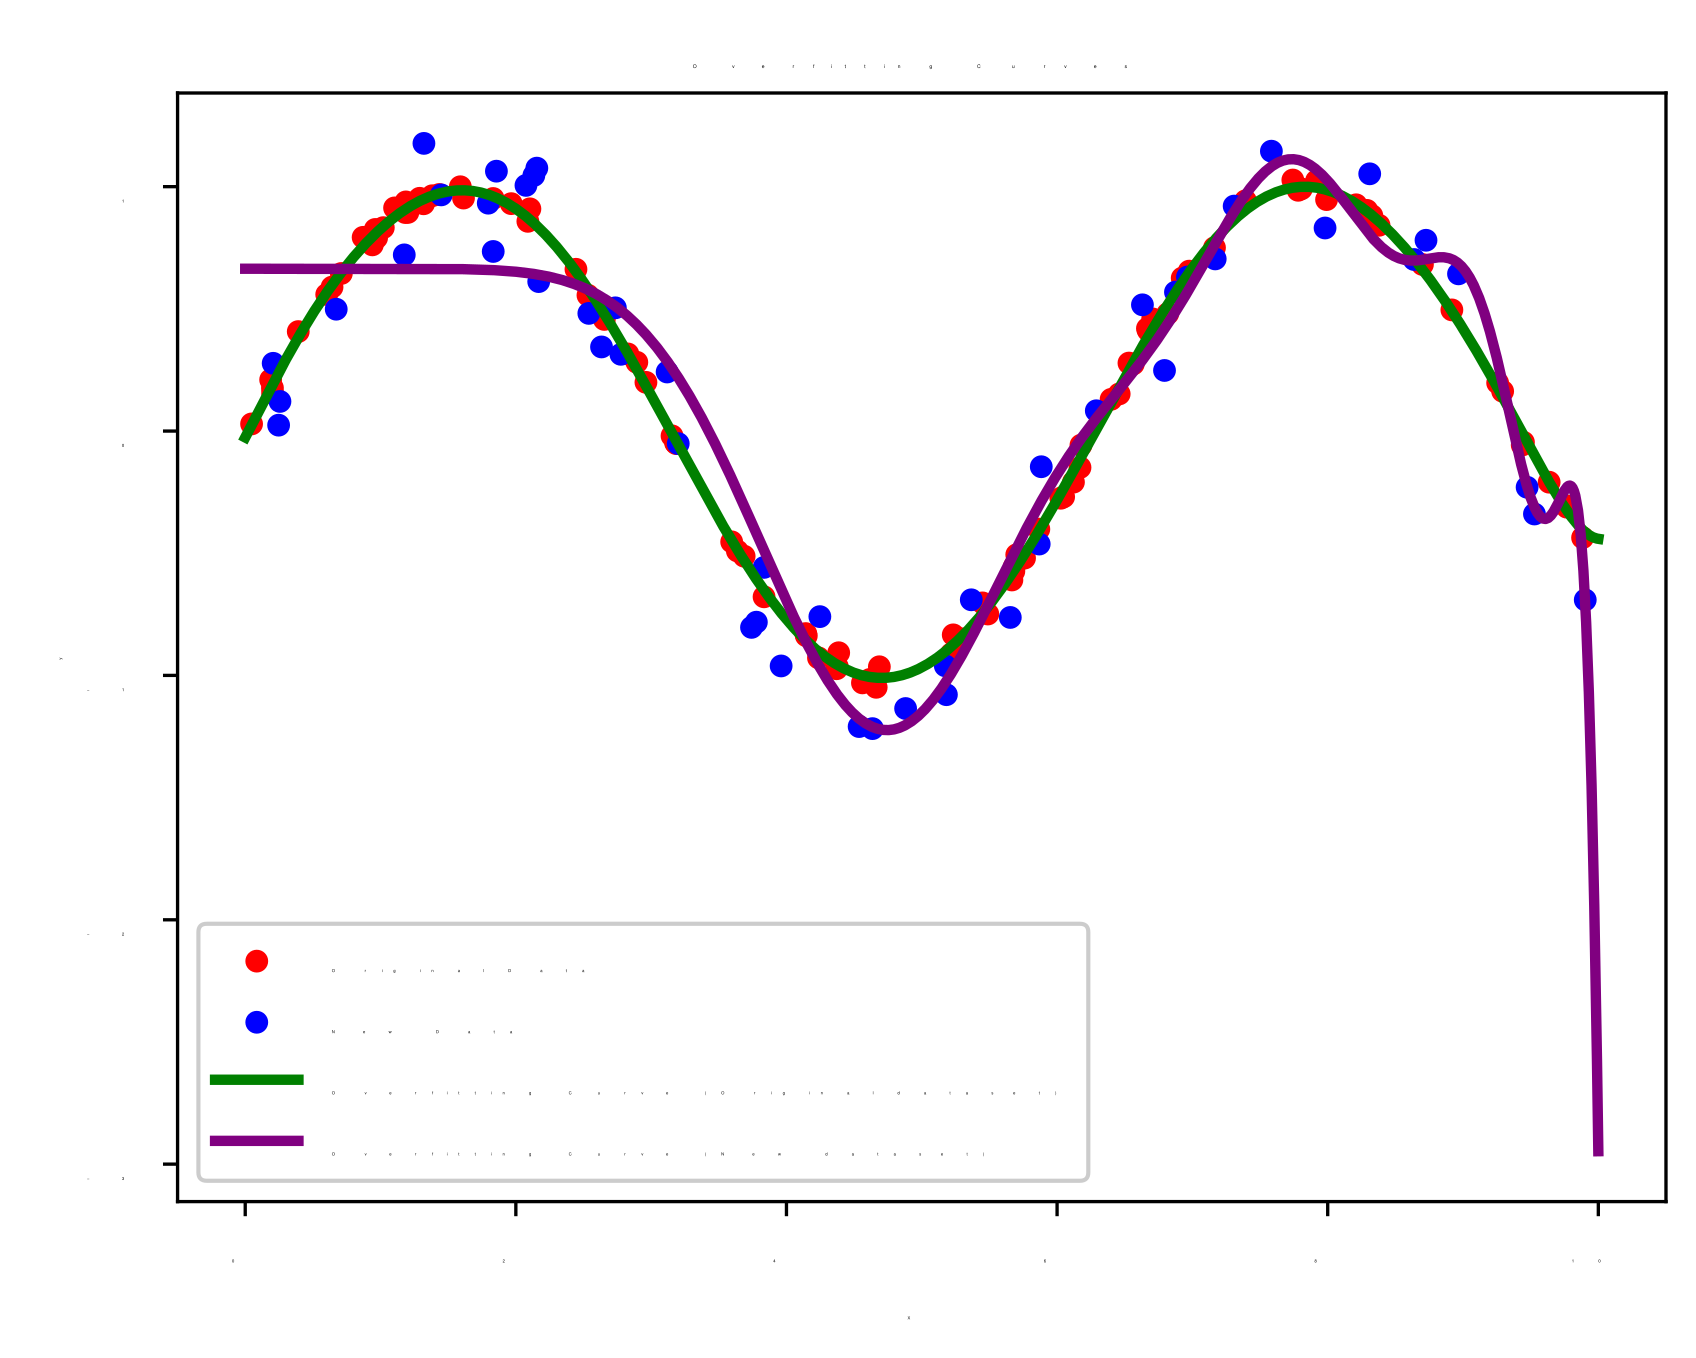
\includegraphics[width=\linewidth]{images/14.png}
    \caption{Over-fitting - High Variance, Low Bias}
  \end{subfigure}%
  \begin{subfigure}{.4\textwidth}
    \centering
    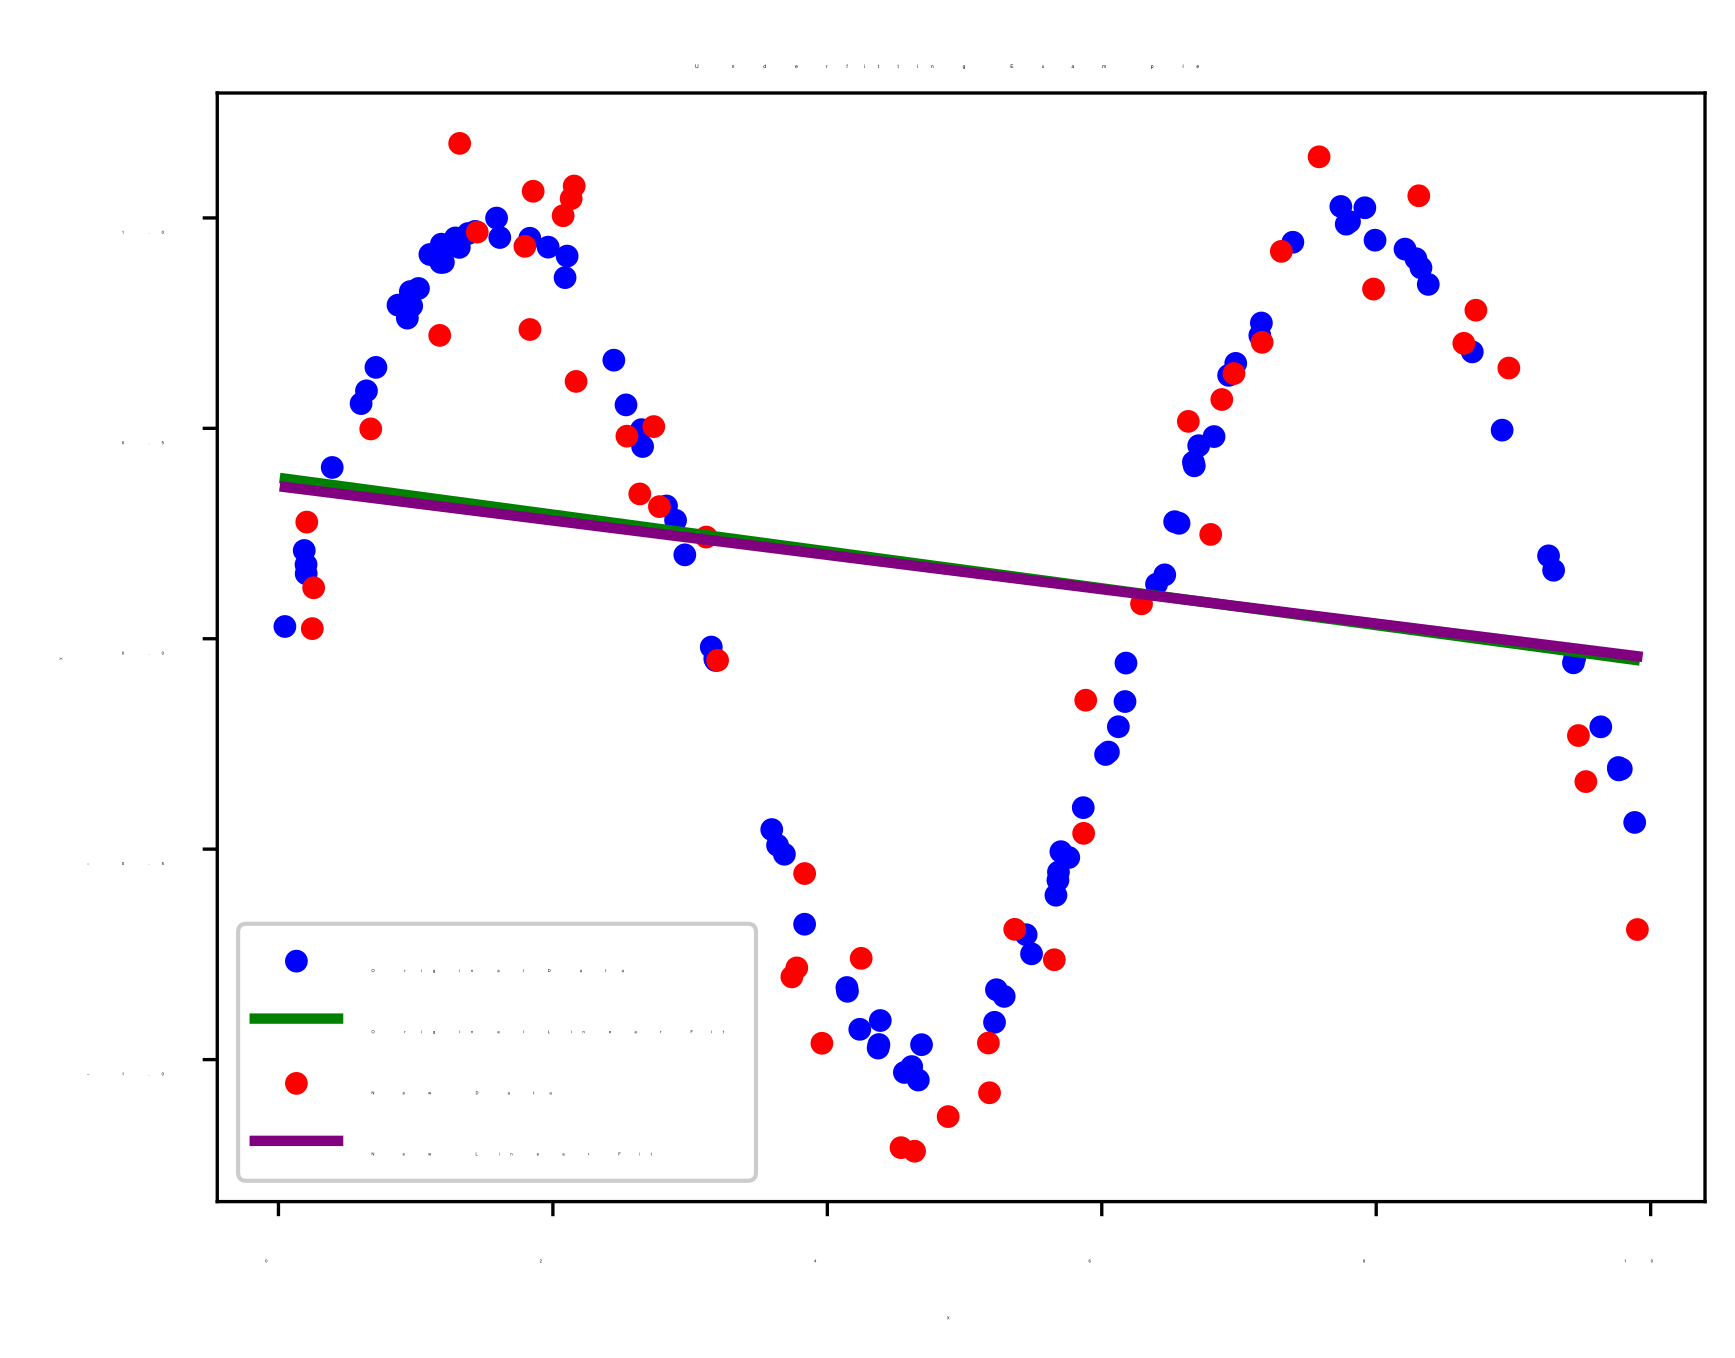
\includegraphics[width=\linewidth]{images/15.png}
    \caption{Under-fitting - Low Variance, High Bias}
  \end{subfigure}
  \caption{Analysing models using bias and variance}
\end{figure}

It is evident that the bias of this high-complexity model is very low. But, as we change the dataset slightly, we can see that there is too much variation in the newly fitted curve. This means that this high-complexity model also has high variance. Similarly, we can consider a low-complexity model such as linear. Here, the predicted values deviate significantly from the actual function, and hence the bias is high. But, changing the dataset has very less effect on the predictor function, suggesting that there is low variance. \\

The ideal model is one that strikes a balance between bias and variance. Highly complex models, like high-order polynomials, may overfit, resulting in \tc{low bias but high variance}. In contrast, lower complexity models might not capture all data complexities, leading to \tc{high bias and low variance}. Both can yield high test errors.

\begin{figure}[H]
  \centering
  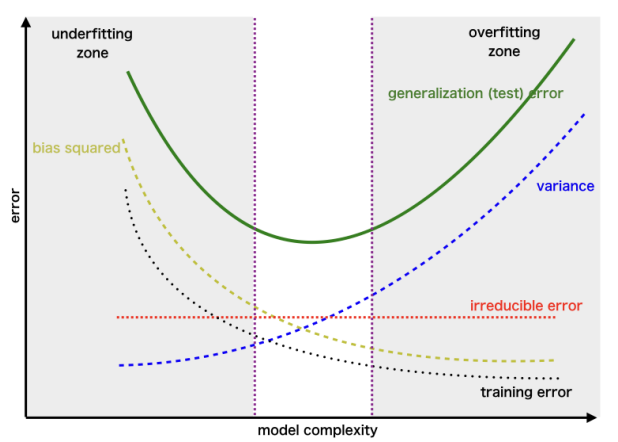
\includegraphics[width = 0.4\textwidth]{images/16.png}
  \caption{Variance Bias Trade-off with Expected Test Error/Generalisation Error}
\end{figure}

Hence, there is an inherent trade-off between variance and bias. We can't make both of them arbitrarily small at the same time. \\

\begin{mdframed}
  Recall $L_2$-Regularised model where,
  $
    \w_{\text{ridge}} = \underset{\w}{\arg\min}
    \left(\norm{y - \mathbf{X}\w}_2^2 + \lambda\norm{\w}_2^2\right)
  $
  . As $\lambda$ increases, the loss penalises high variation of $\w$ and hence the variance decreases. However, this is also reducing the flexibility of model and hence leading to increased bias.
\end{mdframed}